% **** Szablon pracy magisterskiej, licencjackiej lub inżynierskiej ****

\documentclass[polish,12pt,twoside,a4paper]{report}

% *************** Definicje stylu dokumentu ***************

% *********************************************************************************
% W pliku tym zdefiniowany jest wygl¹d dokumentu.
% Zmiany tutaj nie s¹ konieczne o ile nie zamierzasz zmieniaæ wygl¹du dokumentu.
% *********************************************************************************

% *************** Za³adowanie pakietów ***************
\usepackage[a4paper,twoside,left=2.0cm,right=1.5cm,top=1.5cm,bottom=1.5cm]{geometry}
\usepackage[T1]{fontenc}
%\usepackage[cp1250]{inputenc}
\usepackage[utf8]{inputenc}
\usepackage[polish]{babel}
\usepackage{amsmath}
\usepackage{amsfonts}
\usepackage{graphicx}
\usepackage{graphics}
\usepackage{times}
\usepackage{indentfirst}%wciecia a nowych akapitach
\usepackage{listings}
\usepackage{url}
\usepackage[colorlinks=true, linkcolor=black, urlcolor=black, citecolor=black]{hyperref}

\selectlanguage{polish}

%szerokoœœ wciêæ
\setlength{\parindent}{1.25cm}

%numeracja stron
\usepackage{fancyhdr}
\pagestyle{fancy}
\fancyhf{} % usun biezace ustawienia pagin
\fancyhead[LE,RO]{ }
\fancyhead[LO]{ }
\fancyhead[RE]{ }
\fancyfoot[LE,RO]{\small\thepage}
\fancyfoot[LO]{ }
\fancyfoot[RE]{ }
\renewcommand{\headrulewidth}{0.0pt}
\renewcommand{\footrulewidth}{0.0pt}
\addtolength{\headheight}{0.0pt} % pionowy odstep na kreske
\fancypagestyle{plain}{%
\fancyhead{} % usun p. górne na stronach pozbawionych
% numeracji (plain)
\renewcommand{\headrulewidth}{0.0pt} % pozioma kreska
}

% *************** Definicje niektórych kolorów ***************
\usepackage{color}

\definecolor{greenyellow}   {cmyk}{0.15, 0   , 0.69, 0   }
\definecolor{yellow}        {cmyk}{0   , 0   , 1   , 0   }
\definecolor{goldenrod}     {cmyk}{0   , 0.10, 0.84, 0   }
\definecolor{dandelion}     {cmyk}{0   , 0.29, 0.84, 0   }
\definecolor{apricot}       {cmyk}{0   , 0.32, 0.52, 0   }
\definecolor{peach}         {cmyk}{0   , 0.50, 0.70, 0   }
\definecolor{melon}         {cmyk}{0   , 0.46, 0.50, 0   }
\definecolor{yelloworange}  {cmyk}{0   , 0.42, 1   , 0   }
\definecolor{orange}        {cmyk}{0   , 0.61, 0.87, 0   }
\definecolor{burntorange}   {cmyk}{0   , 0.51, 1   , 0   }
\definecolor{bittersweet}   {cmyk}{0   , 0.75, 1   , 0.24}
\definecolor{redorange}     {cmyk}{0   , 0.77, 0.87, 0   }
\definecolor{mahogany}      {cmyk}{0   , 0.85, 0.87, 0.35}
\definecolor{maroon}        {cmyk}{0   , 0.87, 0.68, 0.32}
\definecolor{brickred}      {cmyk}{0   , 0.89, 0.94, 0.28}
\definecolor{red}           {cmyk}{0   , 1   , 1   , 0   }
\definecolor{orangered}     {cmyk}{0   , 1   , 0.50, 0   }
\definecolor{rubinered}     {cmyk}{0   , 1   , 0.13, 0   }
\definecolor{wildstrawberry}{cmyk}{0   , 0.96, 0.39, 0   }
\definecolor{salmon}        {cmyk}{0   , 0.53, 0.38, 0   }
\definecolor{carnationpink} {cmyk}{0   , 0.63, 0   , 0   }
\definecolor{magenta}       {cmyk}{0   , 1   , 0   , 0   }
\definecolor{violetred}     {cmyk}{0   , 0.81, 0   , 0   }
\definecolor{rhodamine}     {cmyk}{0   , 0.82, 0   , 0   }
\definecolor{mulberry}      {cmyk}{0.34, 0.90, 0   , 0.02}
\definecolor{redviolet}     {cmyk}{0.07, 0.90, 0   , 0.34}
\definecolor{fuchsia}       {cmyk}{0.47, 0.91, 0   , 0.08}
\definecolor{lavender}      {cmyk}{0   , 0.48, 0   , 0   }
\definecolor{thistle}       {cmyk}{0.12, 0.59, 0   , 0   }
\definecolor{orchid}        {cmyk}{0.32, 0.64, 0   , 0   }
\definecolor{darkorchid}    {cmyk}{0.40, 0.80, 0.20, 0   }
\definecolor{purple}        {cmyk}{0.45, 0.86, 0   , 0   }
\definecolor{plum}          {cmyk}{0.50, 1   , 0   , 0   }
\definecolor{violet}        {cmyk}{0.79, 0.88, 0   , 0   }
\definecolor{royalpurple}   {cmyk}{0.75, 0.90, 0   , 0   }
\definecolor{blueviolet}    {cmyk}{0.86, 0.91, 0   , 0.04}
\definecolor{periwinkle}    {cmyk}{0.57, 0.55, 0   , 0   }
\definecolor{cadetblue}     {cmyk}{0.62, 0.57, 0.23, 0   }
\definecolor{cornflowerblue}{cmyk}{0.65, 0.13, 0   , 0   }
\definecolor{midnightblue}  {cmyk}{0.98, 0.13, 0   , 0.43}
\definecolor{navyblue}      {cmyk}{0.94, 0.54, 0   , 0   }
\definecolor{royalblue}     {cmyk}{1   , 0.50, 0   , 0   }
\definecolor{blue}          {cmyk}{1   , 1   , 0   , 0   }
\definecolor{cerulean}      {cmyk}{0.94, 0.11, 0   , 0   }
\definecolor{cyan}          {cmyk}{1   , 0   , 0   , 0   }
\definecolor{processblue}   {cmyk}{0.96, 0   , 0   , 0   }
\definecolor{skyblue}       {cmyk}{0.62, 0   , 0.12, 0   }
\definecolor{turquoise}     {cmyk}{0.85, 0   , 0.20, 0   }
\definecolor{tealblue}      {cmyk}{0.86, 0   , 0.34, 0.02}
\definecolor{aquamarine}    {cmyk}{0.82, 0   , 0.30, 0   }
\definecolor{bluegreen}     {cmyk}{0.85, 0   , 0.33, 0   }
\definecolor{emerald}       {cmyk}{1   , 0   , 0.50, 0   }
\definecolor{junglegreen}   {cmyk}{0.99, 0   , 0.52, 0   }
\definecolor{seagreen}      {cmyk}{0.69, 0   , 0.50, 0   }
\definecolor{green}         {cmyk}{1   , 0   , 1   , 0   }
\definecolor{forestgreen}   {cmyk}{0.91, 0   , 0.88, 0.12}
\definecolor{pinegreen}     {cmyk}{0.92, 0   , 0.59, 0.25}
\definecolor{limegreen}     {cmyk}{0.50, 0   , 1   , 0   }
\definecolor{yellowgreen}   {cmyk}{0.44, 0   , 0.74, 0   }
\definecolor{springgreen}   {cmyk}{0.26, 0   , 0.76, 0   }
\definecolor{olivegreen}    {cmyk}{0.64, 0   , 0.95, 0.40}
\definecolor{rawsienna}     {cmyk}{0   , 0.72, 1   , 0.45}
\definecolor{sepia}         {cmyk}{0   , 0.83, 1   , 0.70}
\definecolor{brown}         {cmyk}{0   , 0.81, 1   , 0.60}
\definecolor{tan}           {cmyk}{0.14, 0.42, 0.56, 0   }
\definecolor{gray}          {cmyk}{0   , 0   , 0   , 0.50}
\definecolor{black}         {cmyk}{0   , 0   , 0   , 1   }
\definecolor{white}         {cmyk}{0   , 0   , 0   , 0   } 

% *************** Koniec definicji stylu dokumentu ***************


%definicja przydatnych poleceń
\newcommand{\wydzial}{KOLEGIUM INFORMATYKI STOSOWANEJ}
\newcommand{\kierunek}{Kierunek: INFORMATYKA}
\newcommand{\specjalnosc}{Specjalność: {PROGRAMOWANIE}}
\newcommand{\autor}{Viktor Pylypenko}
\newcommand{\album}{Nr albumu studenta W68166}
\newcommand{\temat}{Aplikacja z interfejsem GUI do zarządzania sklepem z częściami samochodowymi}
\newcommand{\promotor}{mgr inż. Ewa Żesławska}
\newcommand{\typpracy}{Praca projektowa programowanie obiekotwe C\#}
\newcommand{\miasto}{Rzeszów}
\newcommand{\rok}{2025}

\begin{document}

% *************** Włączenie definicji pierwszych stron ***************
% *************** Strony tytułowe ***************

% ************************************************************
% W tym miejscu znajduje sie definicja wyglądu pierwszych stron:
% strony tytułowej, strony z oświadczeniem o treści pracy
% i strony ze spisem treści
% ************************************************************
% *************** Strona tytułowa ***************
%umieszczenie logo i nazwy uczelni
\noindent
\parbox{65mm}{
\includegraphics[width=13.0cm, height=3.0cm]{logoWSIiZ}}

\vspace{10mm}
\begin{center}
{\Large{}\textbf{\wydzial}}
\end{center}
\vspace{10mm}
\noindent
\hspace{30mm}{\Large{}\textbf{\kierunek}}\\

\noindent
\hspace{30mm}{\Large{}\textbf{\specjalnosc}}
\vspace{30mm}
\begin{center}
	{\large{}\autor}\\
	{\large{}\album}\\
	\vspace{15pt}
	{\huge{}\textbf{\textit{\temat}}}\\
	\vspace{20pt}
	{\normalsize{}Prowadzący: \promotor}\\
	\vspace{100pt}
	{\LARGE{}\textbf{\typpracy}}\\
	\vspace{190pt}
	{\large{}\textbf{\miasto {} \rok}}
\end{center}

% pusta zawartość stopki - brak numeru strony
\thispagestyle{empty}

% *************** Strona z oświadczeniem o treści pracy ***************
\newpage
\text{}

\thispagestyle{empty}
\newpage


% *************** Spis treści ***************
\tableofcontents
% pusta zawartość stopki - brak numeru strony
\thispagestyle{empty}
\newpage

% *************** Koniec pliku front.tex ***************



% *************** Część główna pracy ***************
\chapter*{Wstęp}

Projekt „CarParts” ma na celu stworzenie aplikacji służącej do zarządzania częściami samochodowymi, ich kategoriami oraz dostawcami. Głównym celem jest zapewnienie użytkownikom intuicyjnego i prostego w obsłudze interfejsu umożliwiającego zarządzanie informacjami o częściach samochodowych w sposób efektywny i uporządkowany.

Aplikacja wykorzystuje technologie takie jak C\# i ASP.NET Core, co zapewnia stabilność oraz możliwość łatwego skalowania projektu. System pozwala na wykonywanie operacji CRUD na głównych encjach, takich jak Kategorie, Produkty i Dostawcy, a także zapewnia przejrzysty interfejs użytkownika oparty na formularzach graficznych.

 \section*{Założenia projektu}
\begin{enumerate}
    \item Projekt o nazwie \textbf{CarParts} to aplikacja do zarządzania częściami samochodowymi, kategoriami oraz dostawcami, zbudowana w technologii \textbf{C\#} i \textbf{ASP.NET Core}.
    \item Aplikacja umożliwia realizację operacji CRUD (Create, Read, Update, Delete) na encjach: \textbf{Category}, \textbf{Product}, i \textbf{Supplier}.
    \item Interfejs użytkownika jest zbudowany z wykorzystaniem formularzy graficznych \textbf{GUI Forms}, co zapewnia intuicyjne zarządzanie danymi przez użytkownika.
    \item Struktura projektu jest warstwowa, co obejmuje warstwy: \textbf{Controllers}, \textbf{Services}, \textbf{Models}, \textbf{Helpers}, i \textbf{Middleware}.
    \item Dane aplikacji są przechowywane w plikach JSON, zarządzanych przy użyciu klasy \textbf{FileStorageHelper}.
    \item Globalne przetwarzanie wyjątków zostało zaimplementowane w klasie \textbf{ExceptionHandlingMiddleware} dla stabilności systemu.
\end{enumerate}

\section*{Cele projektu}
\begin{enumerate}
    \item Stworzenie skalowalnej i łatwej w utrzymaniu aplikacji do zarządzania częściami samochodowymi.
    \item Zapewnienie użytkownikom możliwości zarządzania kategoriami, produktami oraz dostawcami w sposób intuicyjny i wydajny.
    \item Ułatwienie zarządzania danymi za pomocą graficznego interfejsu użytkownika z obsługą operacji CRUD.
    \item Wdrożenie dobrej praktyki projektowania, opartej na podejściu warstwowym, aby oddzielić logikę biznesową od prezentacji i danych.
    \item Zastosowanie narzędzi takich jak \textbf{Swagger} dla automatycznej dokumentacji API.
\end{enumerate}
\newpage


\addcontentsline{toc}{chapter}{Wstęp}
\newpage
% ********** Rozdział 1 ********** \chapter{Opis założeń projektu} \section{Cele projektu}


\chapter{Wymagania funkcjonalne i niefunkcjonalne} \noindent \section{Wymagania funkcjonalne} \begin{itemize} \item System umożliwia operacje CRUD na encjach: \begin{itemize} \item Kategorie (Category) – zarządzanie nazwą i opisem. \item Produkty (Product) – zarządzanie nazwą, ceną, kodem oraz powiązaniem z kategorią i dostawcą. \item Dostawcy (Supplier) – zarządzanie nazwą, informacjami kontaktowymi oraz adresem. \end{itemize} \item Intuicyjny interfejs użytkownika pozwala na przeglądanie, dodawanie, edytowanie oraz usuwanie danych. \item Walidacja danych wejściowych, np. ograniczenie zakresu cen czy maksymalna długość pól tekstowych. \item Obsługa API, umożliwiająca komunikację z backendem za pomocą klasy HttpClient. \item Przechowywanie danych w plikach JSON. \end{itemize}

\noindent \section{Wymagania niefunkcjonalne:} \begin{itemize} \item \textbf{Wydajność:} Operacje CRUD muszą działać z minimalnym opóźnieniem. \item \textbf{Skalowalność:} Struktura projektu umożliwia dodawanie nowych funkcjonalności. \item \textbf{Stabilność:} Obsługa wyjątków chroni system przed błędami krytycznymi. \item \textbf{Przenośność:} Kompatybilność z każdym systemem obsługującym środowisko .NET Core. \item \textbf{Bezpieczeństwo:} Walidacja danych chroni przed błędami i nieprawidłowymi danymi. \item \textbf{Dostępność:} Intuicyjny GUI ułatwia obsługę aplikacji przez użytkowników bez zaawansowanej wiedzy technicznej. \end{itemize}


% ********** Koniec rozdziału **********
\newpage
% ********** Rozdział 2 **********
\chapter{Opis struktury projektu}

\section{Struktura i Opis Techniczny}
System został zaprojektowany w oparciu o architekturę warstwową, składającą się z następujących komponentów:
\begin{itemize}
    \item Warstwa Kontrolerów: Obsługuje zapytania HTTP i deleguje logikę do odpowiednich usług.
    \item Warstwa Usług: Implementuje logikę biznesową, operując na danych i koordynując interakcje z bazą danych.
    \item Warstwa Modeli: Definiuje struktury danych używane w systemie.
    \item Baza Danych: Przechowuje dane systemowe w formacie JSON, korzystając z plików jako persystencji.
\end{itemize}

\section{Język, Narzędzia i Wymagania Sprzętowe}
\subsection{Język Programowania}
System został zaimplementowany w języku \textbf{C\#} z wykorzystaniem frameworka \textbf{ASP.NET Core}.

\subsection{Narzędzia}
\begin{itemize}
    \item IDE: Microsoft Visual Studio
    \item Biblioteki: Newtonsoft.Json (do operacji na danych JSON)
    \item Serwer: Kestrel wbudowany w ASP.NET Core
    \item Testowanie: Swagger UI dla testowania API
\end{itemize}

\subsection{Minimalne Wymagania Sprzętowe}
\begin{itemize}
    \item Procesor: Dual-core 2 GHz lub lepszy
    \item RAM: 4 GB
    \item Dysk: 100 MB wolnego miejsca
    \item System Operacyjny: Windows 10 lub nowszy
\end{itemize}

\section{Zarządzanie Danymi i Baza Danych}
Dane w systemie przechowywane są w formacie JSON w plikach:
\begin{itemize}
    \item \texttt{categories.txt} - kategorie produktów
    \item \texttt{products.txt} - produkty
    \item \texttt{suppliers.txt} - dostawcy
\end{itemize}

Operacje na danych realizowane są za pomocą klasy \texttt{FileStorageHelper}, która umożliwia odczyt i zapis danych JSON.

\section{Hierarchia Klas i Kluczowe Metody}
Hierarchia klas została zaprojektowana w sposób modularny i rozszerzalny. Kluczowe klasy to:

\subsection{Klasa \texttt{Category}}
Definicja kategorii produktów.
\begin{itemize}
    \item \textbf{Właściwości:}
    \begin{itemize}
        \item \texttt{Id} - identyfikator kategorii
        \item \texttt{Name} - nazwa kategorii
        \item \texttt{Description} - opis kategorii
    \end{itemize}
\end{itemize}

\subsection{Klasa \texttt{CategoryService}}
Implementacja logiki biznesowej dla kategorii.
\begin{itemize}
    \item \texttt{GetAllCategories()} - zwraca wszystkie kategorie.
    \item \texttt{GetCategoryById(int id)} - zwraca kategorię na podstawie \texttt{Id}.
    \item \texttt{AddCategory(Category category)} - dodaje nową kategorię.
    \item \texttt{UpdateCategory(int id, Category category)} - aktualizuje istniejącą kategorię.
    \item \texttt{DeleteCategory(int id)} - usuwa kategorię.
\end{itemize}

\subsection{Klasa \texttt{Product}}
Definicja produktu.
\begin{itemize}
    \item \textbf{Właściwości:}
    \begin{itemize}
        \item \texttt{Id} - identyfikator produktu
        \item \texttt{Name} - nazwa produktu
        \item \texttt{Price} - cena produktu
        \item \texttt{Code} - kod produktu
    \end{itemize}
\end{itemize}

\subsection{Klasa \texttt{ProductService}}
Logika biznesowa dla produktów.
\begin{itemize}
    \item \texttt{GetAllProducts()} - zwraca wszystkie produkty.
    \item \texttt{AddProduct(Product product)} - dodaje nowy produkt.
    \item \texttt{UpdateProduct(int id, Product product)} - aktualizuje istniejący produkt.
\end{itemize}

\subsection{Klasa \texttt{Supplier}}
Definicja dostawcy.
\begin{itemize}
    \item \textbf{Właściwości:}
    \begin{itemize}
        \item \texttt{Id} - identyfikator dostawcy
        \item \texttt{Name} - nazwa dostawcy
        \item \texttt{ContactInfo} - informacje kontaktowe
        \item \texttt{Address} - adres
    \end{itemize}
\end{itemize}

\subsection{Klasa \texttt{SupplierService}}
Logika biznesowa dla dostawców.
\begin{itemize}
    \item \texttt{GetAllSuppliers()} - zwraca wszystkich dostawców.
    \item \texttt{AddSupplier(Supplier supplier)} - dodaje nowego dostawcę.
    \item \texttt{UpdateSupplier(int id, Supplier supplier)} - aktualizuje dane dostawcy.
\end{itemize}

% ********** Koniec rozdziału **********

\newpage
% ********** Rozdział 4 **********
\chapter{Harmonogram realizacji projektu}

\section{Harmonogram realizacji}

W celu zaplanowania i monitorowania postępów w realizacji projektu został stworzony diagram Gantta, który przedstawia podział projektu na poszczególne etapy i terminy ich realizacji. Diagram ten jest przedstawiony na rysunku \ref{fig:gantt}.

\begin{figure}[h!]
    \centering
    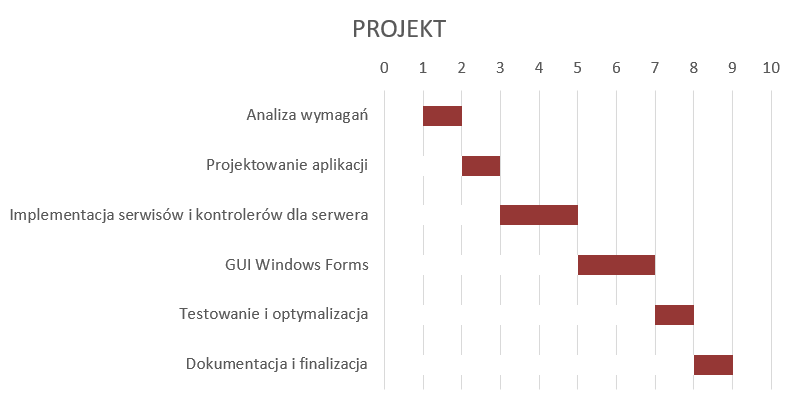
\includegraphics[width=\textwidth]{figures/diagram.png}
    \caption{Diagram Gantta przedstawiający harmonogram realizacji projektu.}
    \label{fig:gantt}
\end{figure}

Diagram obejmuje następujące etapy:
\begin{enumerate}
    \item \textbf{Analiza wymagań (tygodnie 1-2):} Na tym etapie zebrano wymagania i przygotowano ogólną koncepcję projektu.
    \item \textbf{Projektowanie aplikacji (tygodnie 2-3):} Opracowano architekturę systemu, w tym schematy baz danych i strukturę kodu.
    \item \textbf{Implementacja serwisów i kontrolerów dla serwera (tygodnie 3-5):} Zaimplementowano backend aplikacji z wykorzystaniem API.
    \item \textbf{GUI Windows Forms (tygodnie 5-7):} Stworzono graficzny interfejs użytkownika, umożliwiający interakcję z systemem.
    \item \textbf{Testowanie i optymalizacja (tygodnie 7-8):} Przeprowadzono testy jednostkowe i integracyjne, wprowadzono poprawki oraz zoptymalizowano kod.
    \item \textbf{Dokumentacja i finalizacja (tygodnie 8-9):} Przygotowano dokumentację użytkownika i kodu oraz sfinalizowano projekt.
\end{enumerate}

\section{Repozytorium i system kontroli wersji}

Kod źródłowy projektu został umieszczony w publicznie dostępnym repozytorium na platformie GitHub. Repozytorium dostępne jest pod adresem w załączniku.


W projekcie wykorzystano system kontroli wersji \textbf{Git}, który umożliwia:
\begin{itemize}
    \item Śledzenie historii zmian w kodzie.
    \item Współpracę zespołową poprzez rozgałęzienia (\textit{branches}) i scalanie (\textit{merge}).
    \item Szybkie cofanie wprowadzonych zmian w przypadku wykrycia błędów.
\end{itemize}

\textbf{Struktura repozytorium:}  
Struktura repozytorium odpowiada strukturze projektu opisanej w poprzednich rozdziałach

% ********** Koniec rozdziału **********
\newpage
% ********** Rozdział 4 **********
\chapter{Prezentacja warstwy użytkowej projektu}
\section{Zrzuty ekranu aplikacji i ich opisy}

Poniżej znajduje się zestaw zrzutów ekranu przedstawiających różne funkcje i operacje w Panelu Kontrolnym Dostawców. W panelu wyróżniono następujące sekcje:
\begin{itemize}
    \item Pierwszy textbox i zielony przycisk: \textbf{Załaduj listę dostawców}.
    \item Drugi textbox i niebieski przycisk: \textbf{Dodaj nowego dostawcę}.
    \item Trzeci textbox i niebieski przycisk: \textbf{Aktualizuj dane istniejącego dostawcy}.
    \item Czwarty textbox i czerwony przycisk: \textbf{Usuń dostawcę według ID}.
\end{itemize}

\subsection{Funkcjonalności panelu}
W aplikacji główny widok umożliwia wykonywanie podstawowych operacji CRUD (Create, Read, Update, Delete) na danych dostawców. Na przykład, na rysunku \ref{fig:suppliers_test_1} widzimy ekran startowy panelu, gdzie możemy załadować listę dostawców przy użyciu zielonego przycisku. Po wczytaniu danych, jak na rysunku \ref{fig:suppliers_test_2}, użytkownik może przystąpić do dodawania, modyfikacji lub usuwania danych.

Na rysunku \ref{fig:suppliers_test_3} zaprezentowano przykład dodawania nowego dostawcy, gdzie w drugim textboxie należy wprowadzić szczegóły, a następnie kliknąć \textbf{Dodaj}. System wyświetla potwierdzenie sukcesu operacji, jak pokazano na rysunku \ref{fig:suppliers_test_4}.

Z kolei na rysunku \ref{fig:suppliers_test_6} pokazano możliwość aktualizacji danych istniejącego dostawcy, za pomocą trzeciego textboxa i przycisku \textbf{Aktualizuj}. Po dokonaniu zmian lista dostawców zostaje odświeżona, co widać na rysunku \ref{fig:suppliers_test_7}. Dodatkowo użytkownik może usuwać dostawców, podając ich ID w czwartym textboxie i klikając czerwony przycisk, jak pokazano na rysunku \ref{fig:suppliers_test_8}.

W przypadku błędów, takich jak nieprawidłowe dane wejściowe, aplikacja wyświetla odpowiednie komunikaty, co przedstawiono na rysunku \ref{fig:suppliers_test_9_1}.

\subsection{Rozszerzenia aplikacji}
Poza obsługą dostawców aplikacja zawiera panele umożliwiające zarządzanie produktami i kategoriami. Jak widać na rysunku \ref{fig:suppliers_test_10}, panel produktów działa na podobnych zasadach, umożliwiając dodawanie, modyfikację i usuwanie danych produktów. Panel kategorii, przedstawiony na rysunku \ref{fig:suppliers_test_11}, pozwala na podobne operacje w kontekście zarządzania kategoriami.

\subsection{Dokumentacja API}
Rysunek \ref{fig:swagger} przedstawia dokumentację API wygenerowaną za pomocą narzędzia Swagger. Dzięki tej dokumentacji możliwe jest łatwe zrozumienie struktury zapytań i odpowiedzi w aplikacji. API zostało zaprojektowane w sposób uniwersalny, umożliwiając interakcję z backendem nie tylko za pomocą aplikacji napisanej w Windows Forms, ale również przy użyciu dowolnej platformy czy frameworka, takich jak:
\begin{itemize}
    \item aplikacje webowe oparte na frameworkach takich jak \textbf{React}, \textbf{Angular} czy \textbf{Vue.js},
    \item aplikacje mobilne tworzone w \textbf{Flutter}, \textbf{React Native} lub \textbf{Swift},
    \item aplikacje desktopowe budowane z użyciem innych frameworków.
\end{itemize}

Dzięki temu podejściu frontend może być dostosowany do różnych potrzeb użytkowników, co znacząco zwiększa wszechstronność i skalowalność rozwiązania. Przykładowo, firma może zaimplementować aplikację mobilną do szybkiego zarządzania dostawcami, podczas gdy inny zespół pracuje nad rozbudowaną aplikacją webową dla większych operacji.

\subsection{Zrzuty ekranu}

\begin{figure}[h!]
    \centering
    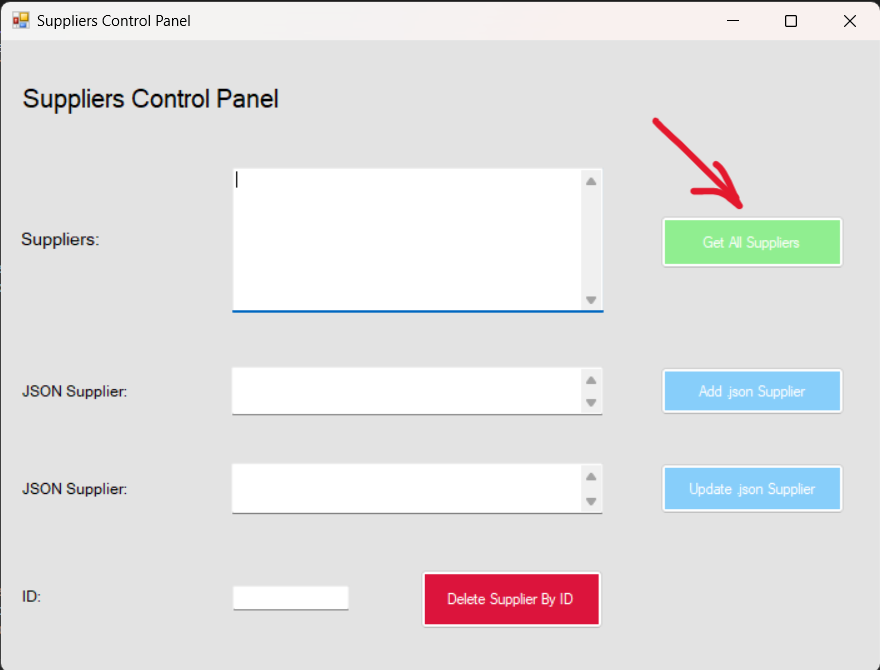
\includegraphics[width=0.8\textwidth]{img_tests/suppliers_test_1.png}
    \caption{Ekran startowy panelu. Funkcja załaduj listę dostawców za pomocą zielonego przycisku.}
    \label{fig:suppliers_test_1}
\end{figure}

\begin{figure}[h!]
    \centering
    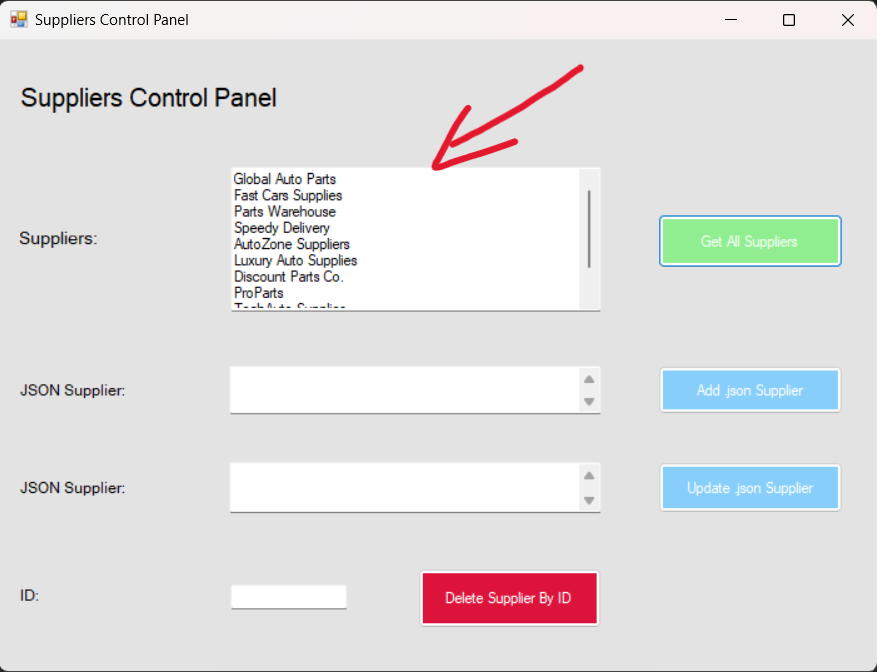
\includegraphics[width=0.8\textwidth]{img_tests/suppliers_test_2.png}
    \caption{Lista dostawców załadowana w pierwszym polu tekstowym po kliknięciu przycisku \textbf{Załaduj}.}
    \label{fig:suppliers_test_2}
\end{figure}

\begin{figure}[h!]
    \centering
    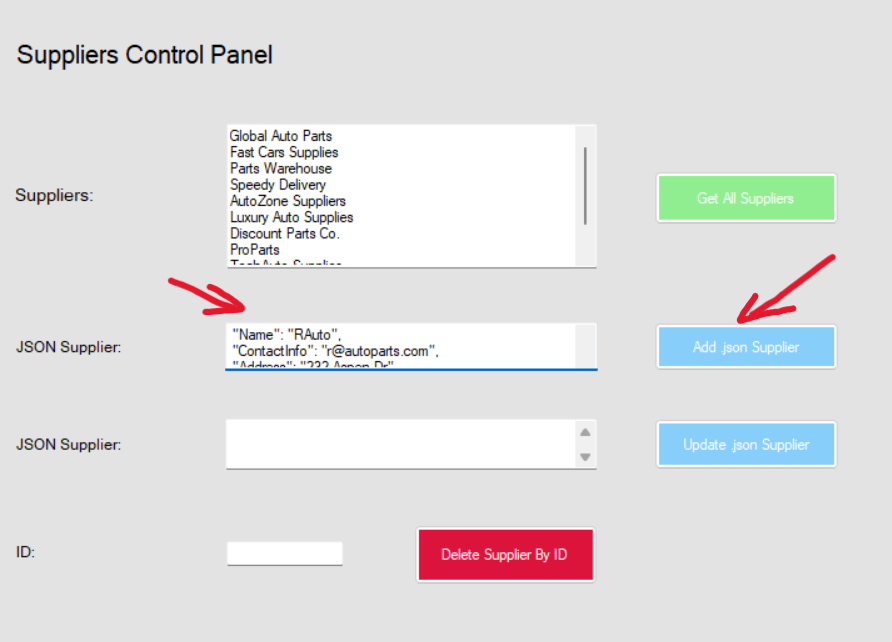
\includegraphics[width=0.8\textwidth]{img_tests/suppliers_test_3.png}
    \caption{Dodawanie nowego dostawcy. Drugi tekstboks służy do wprowadzania danych nowego dostawcy. Kliknij \textbf{Dodaj}, aby zatwierdzić.}
    \label{fig:suppliers_test_3}
\end{figure}

\begin{figure}[h!]
    \centering
    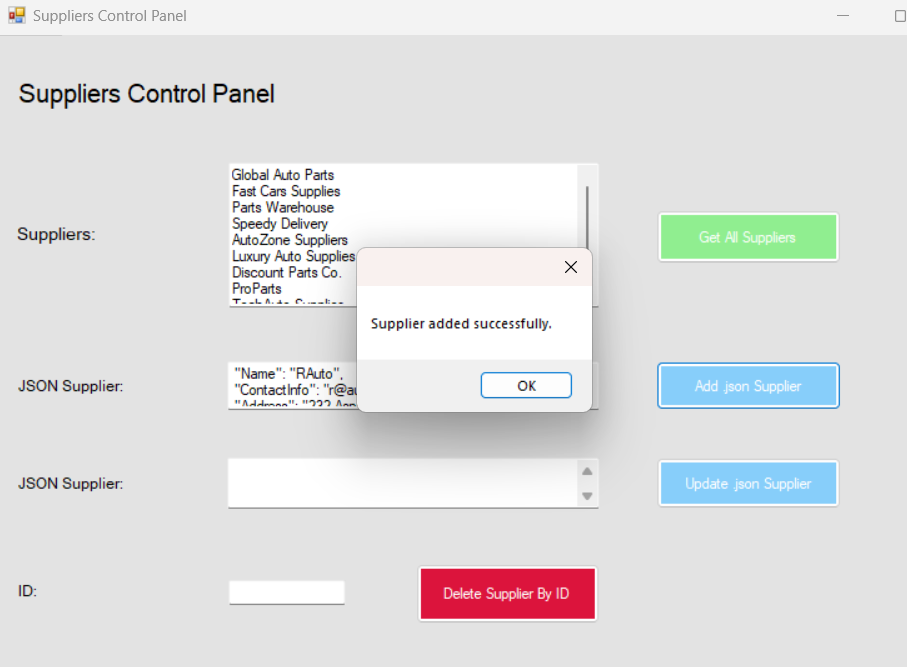
\includegraphics[width=0.8\textwidth]{img_tests/suppliers_test_4.png}
    \caption{Potwierdzenie pomyślnego dodania nowego dostawcy.}
    \label{fig:suppliers_test_4}
\end{figure}

\begin{figure}[h!]
    \centering
    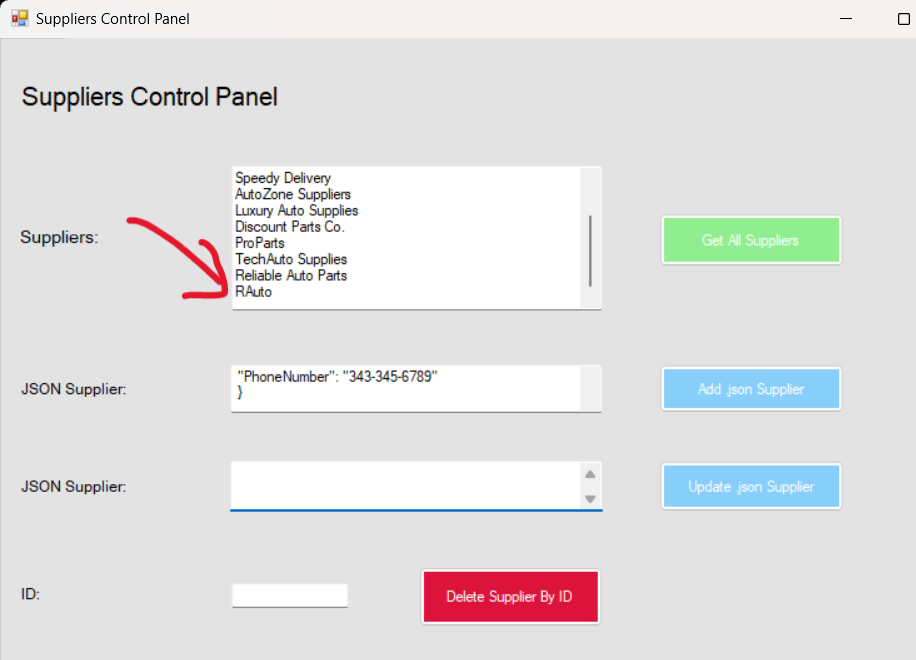
\includegraphics[width=0.8\textwidth]{img_tests/suppliers_test_5.png}
    \caption{Potwierdzenie pomyślnego dodania nowego dostawcy.}
    \label{fig:suppliers_test_5}
\end{figure}

\begin{figure}[h!]
    \centering
    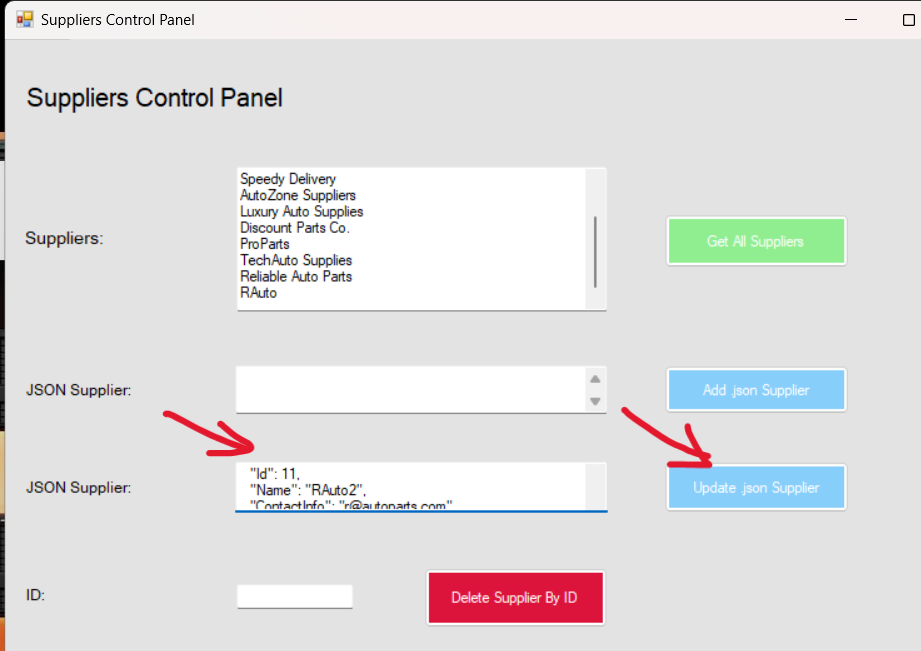
\includegraphics[width=0.8\textwidth]{img_tests/suppliers_test_6.png}
    \caption{Wprowadzanie danych dostawcy do aktualizacji w trzecim tekście i zatwierdzanie przyciskiem \textbf{Aktualizuj}.}
    \label{fig:suppliers_test_6}
\end{figure}

\begin{figure}[h!]
    \centering
    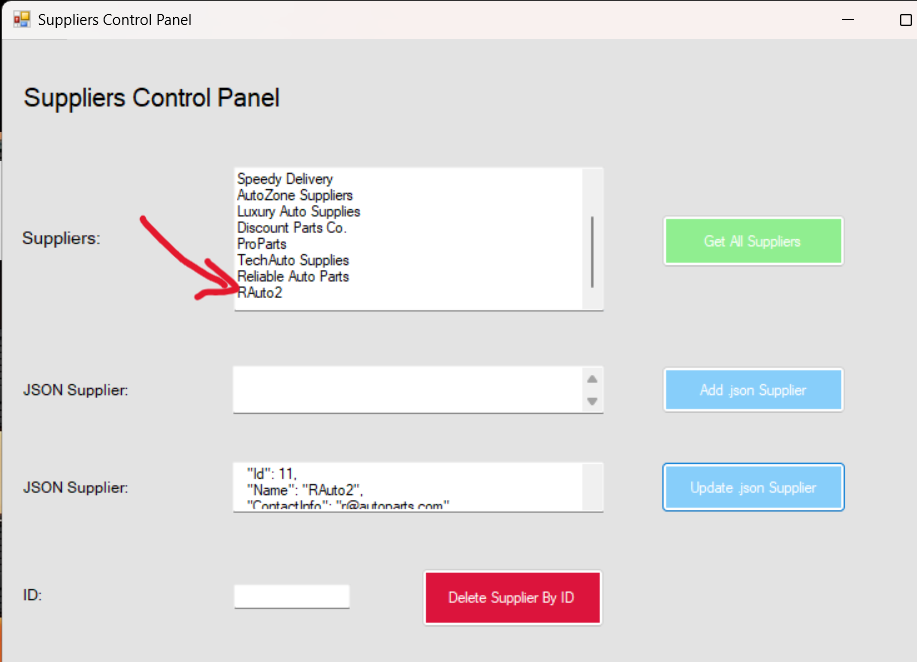
\includegraphics[width=0.8\textwidth]{img_tests/suppliers_test_7.png}
    \caption{Lista dostawców wczytana po modyfikacji z możliwością usunięcia rekordu po ID.}
    \label{fig:suppliers_test_7}
\end{figure}

\begin{figure}[h!]
    \centering
    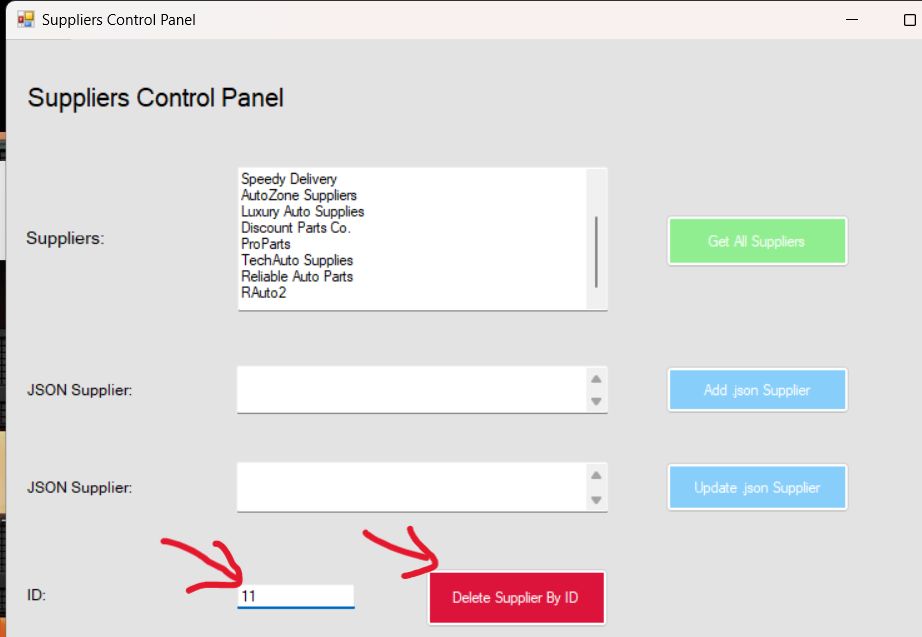
\includegraphics[width=0.8\textwidth]{img_tests/suppliers_test_8.png}
    \caption{Usunięcie dostawcy po ID za pomocą czwartego tekstowego pola i czerwonego przycisku \textbf{Usuń}.}
    \label{fig:suppliers_test_8}
\end{figure}

\begin{figure}[h!]
    \centering
    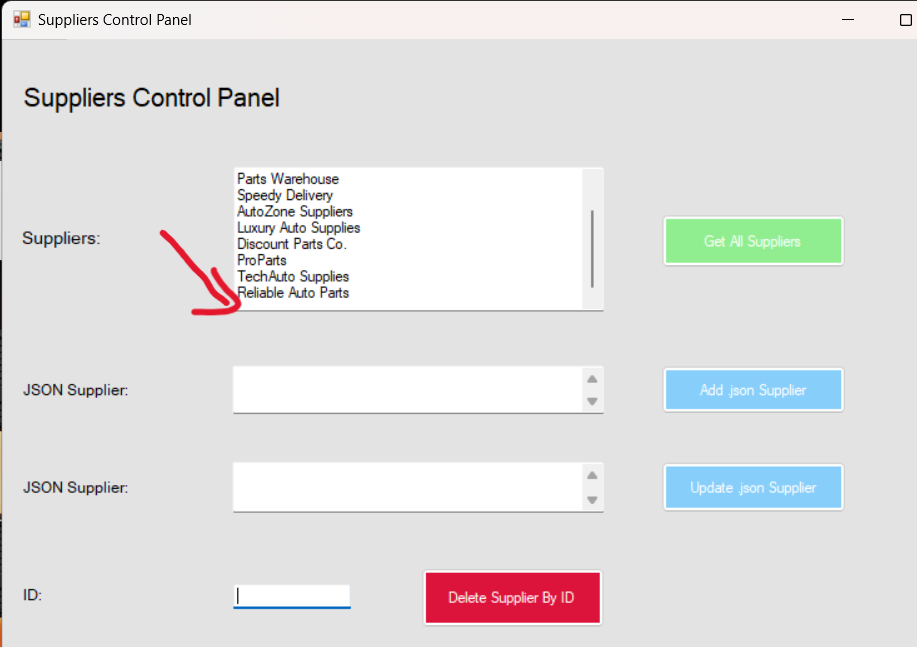
\includegraphics[width=0.8\textwidth]{img_tests/suppliers_test_9.png}
    \caption{Wyświetlenie danych po usunięciu.}
    \label{fig:suppliers_test_9}
\end{figure}

\begin{figure}[h!]
    \centering
    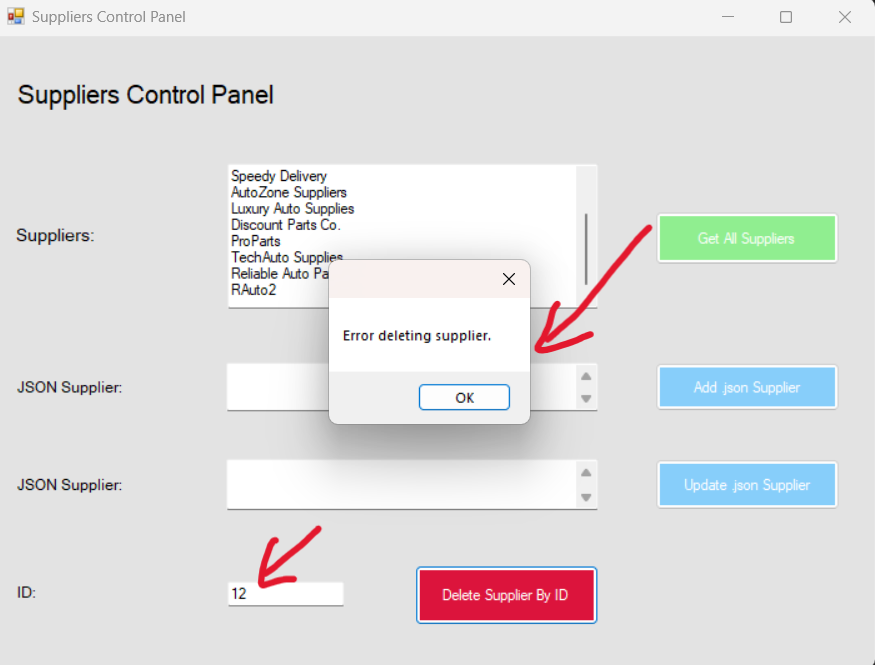
\includegraphics[width=0.8\textwidth]{img_tests/suppliers_test_9_1.png}
    \caption{Wyświetlenie błędu lub informacji o nieprawidłowych danych wprowadzonego dostawcy.}
    \label{fig:suppliers_test_9_1}
\end{figure}


\begin{figure}[h!]
    \centering
    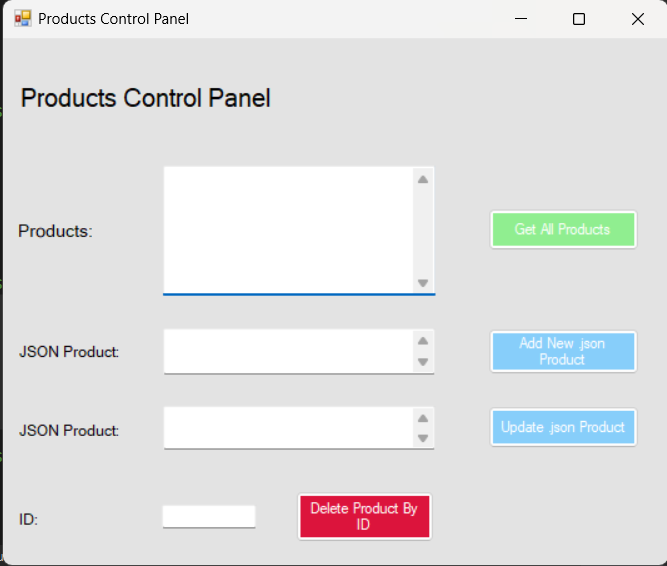
\includegraphics[width=0.8\textwidth]{img_tests/suppliers_test_10.png}
    \caption{Panel zarządzania produktami z funkcjami podobnymi do Panelu Dostawców.}
    \label{fig:suppliers_test_10}
\end{figure}

\begin{figure}[h!]
    \centering
    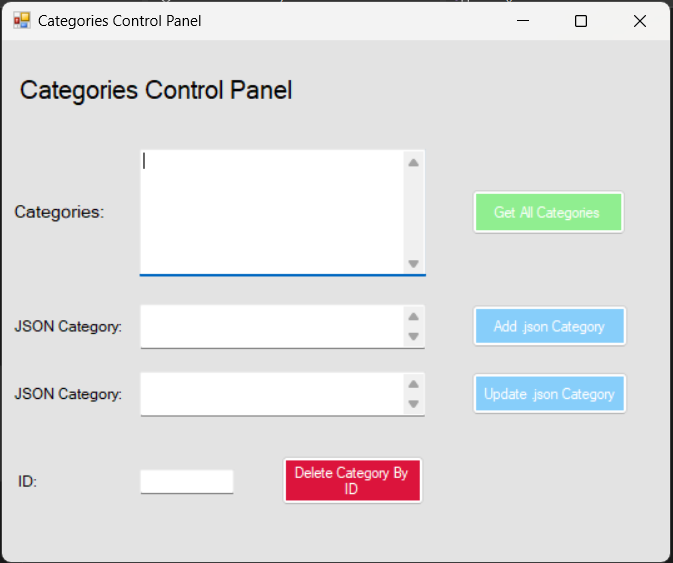
\includegraphics[width=0.8\textwidth]{img_tests/suppliers_test_11.png}
    \caption{Panel zarządzania kategoriami z możliwością dodawania, aktualizowania i usuwania kategorii.}
    \label{fig:suppliers_test_11}
\end{figure}

\begin{figure}[h!]
    \centering
    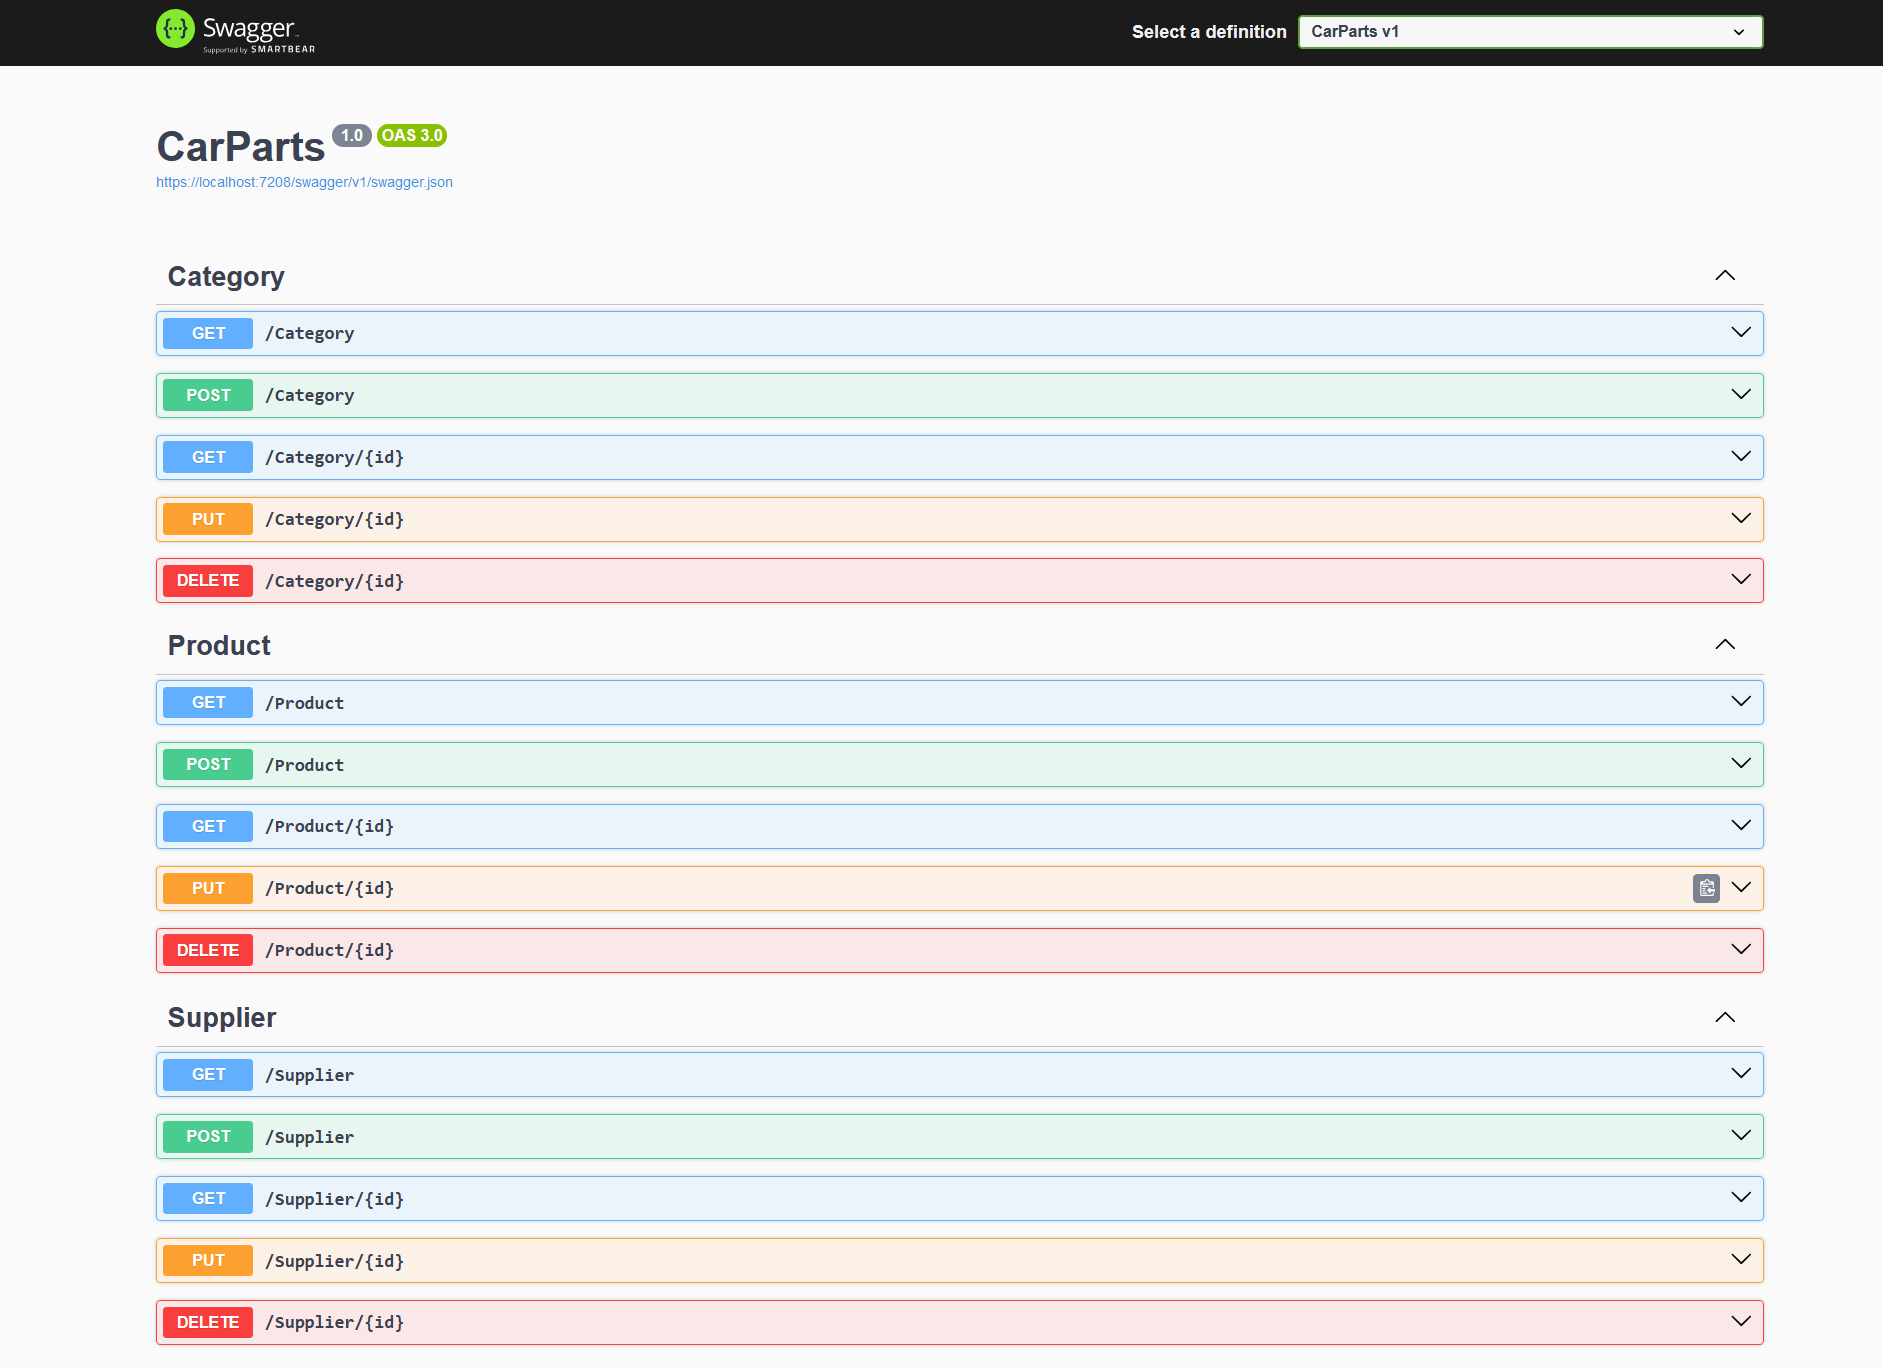
\includegraphics[width=0.8\textwidth]{img_tests/swagger.png}
    \caption{Widok dokumentacji API (Swagger) dla interakcji z backendem aplikacji.}
    \label{fig:swagger}
\end{figure}
% ********** Koniec rozdziału **********
\newpage
\chapter{Podsumowanie}

W ramach projektu zrealizowano wszystkie zaplanowane etapy, obejmujące analizę, projektowanie oraz implementację aplikacji. Ostatecznym rezultatem jest funkcjonalna aplikacja desktopowa do zarządzania sklepem z częściami samochodowymi, wykorzystująca technologię Windows Forms i backend oparty na REST API. Aplikacja została zintegrowana z systemem kontroli wersji Git, a jej kod źródłowy umieszczono w publicznym repozytorium.

\section{Zrealizowane prace}
\begin{enumerate}
    \item \textbf{Analiza wymagań}: Zidentyfikowano kluczowe funkcjonalności aplikacji, takie jak zarządzanie dostawcami, produktami i kategoriami.
    \item \textbf{Projektowanie aplikacji}: Przygotowano strukturę aplikacji, diagramy klas i przepływu danych.
    \item \textbf{Implementacja serwisów i kontrolerów}: Zrealizowano backend z wykorzystaniem .NET.
    \item \textbf{Interfejs użytkownika}: Stworzono GUI w technologii Windows Forms, zapewniające intuicyjność i wygodę użytkowania.
    \item \textbf{Testowanie i optymalizacja}: Przeprowadzono testy jednostkowe i integracyjne oraz optymalizację wydajności.
    \item \textbf{Dokumentacja}: Przygotowano dokumentację projektu, w tym diagramy Gantta i szczegółowy opis funkcjonalności.
\end{enumerate}

\section{Możliwości dalszego rozwoju}
Aplikacja jest modułowa i pozwala na łatwy rozwój. Możliwe kierunki rozwoju to:
\begin{itemize}
     \item Rozbudowa bazy danych o nowe modele i specyficzne funkcje w endpointach API.
    \item Migracja na aplikację webową z użyciem nowoczesnych frameworków.
    \item Rozszerzenie funkcjonalności o generowanie raportów, analizy danych czy powiadomienia email.
    \item Stworzenie wersji mobilnej z wykorzystaniem Xamarin lub Flutter.
    \item Ulepszenie UX/UI z wykorzystaniem nowoczesnych bibliotek graficznych.
\end{itemize}

\section{Podsumowanie końcowe}
Projekt został zrealizowany zgodnie z założeniami i harmonogramem. Aplikacja spełnia wymagania i jest gotowa do dalszego rozwoju. Modularność i użyte technologie umożliwiają łatwą adaptację do zmieniających się potrzeb i rozbudowy funkcjonalności, co stanowi solidną podstawę do wdrożenia w środowisku produkcyjnym.

\newpage


% *************** Bibliografia ***************
\begin{thebibliography}{6}
\addcontentsline{toc}{chapter}{Bibliografia}
%dodanie wpisu do spisu bibliograficznego

\bibitem{swagger} Swagger Documentation, \textit{https://swagger.io/docs/}, dostęp: 20.01.2025.
\bibitem{dotnet} Microsoft, \textit{ASP.NET Core Documentation}, Microsoft, dostęp: 20.01.2025.
\bibitem{rest-api} Fielding, R. T., \textit{Architectural Styles and the Design of Network-based Software Architectures}, University of California, 2000.
\bibitem{windows-forms} Microsoft, \textit{Windows Forms Documentation}, Microsoft, dostęp: 20.01.2025.
\bibitem{git} Git Documentation, \textit{https://git-scm.com/doc}, dostęp: 20.01.2025.

\end{thebibliography}
\newpage

% *************** Zakończenie ***************
% *************** Zakończenie ***************

%***************************************************************************************
% W tym miejscu znajdują się polecenia odpowiedzialne za tworzenie
% spisu ilustracji, spisu treści oraz streszczenia pracy
%***************************************************************************************

%spis rysunków
\addcontentsline{toc}{chapter}{Spis rysunków}
\listoffigures
\newpage



% %streszczenie
% \addcontentsline{toc}{chapter}{Streszczenie}
% \noindent
% {\footnotesize{}\textbf{Wyższa Szkoła Informatyki i Zarządzania z siedzibą w Rzeszowie\\
% Kolegium Informatyki Stosowanej}
% \vspace{30pt}

% \begin{center}
% \textbf{Streszczenie pracy dyplomowej inżynierskiej}\\
% \temat
% \end{center}

% \vspace{30pt}
% \noindent
% \textbf{Autor: \autor
% \\Promotor: \promotor
% \\Słowa kluczowe: tutaj umieść słowa kluczowe}
% \vspace{40pt}
% \\Treść streszczenia, czyli kilka zdań dotyczących treści pracy dyplomowej w języku polskim.
% \vspace{80pt}

% \noindent
% \textbf{The University of Information Technology and Management in Rzeszow\\
% Faculty of Applied Information Technology}
% \vspace{30pt}

% \begin{center}
% \textbf{Thesis Summary\\}
% Tytuł pracy w języku angielskim
% \end{center}

% \vspace{30pt}
% \noindent
% \textbf{Author: \autor
% \\Supervisor: \promotor
% \\Key words: tutaj umieść słowa kluczowe}
% \vspace{40pt}
% \\Treść streszczenia, czyli kilka zdań dotyczących treści pracy dyplomowej w języku angielskim - tłumaczenie tekstu z języka polskiego.
% }

% *************** Koniec pliku back.tex ***************


\end{document}
% *************** Koniec pliku szablon.tex ***************